\section{Explainability of Neural Networks}
Neural networks (NNs) have become one of significant machine learning algorithms that successfully underpin applications in various domains, such as  computer vision and NLP. Despite the achievements, they are still considered as black box processes where their predictions are difficult to be interpreted by  humans. In particular, we barely know the evidence how the networks transform input to such accurate predictions.

%\begin{figure}
%  \centering
%  \begin{minipage}{\textwidth}
%  
%			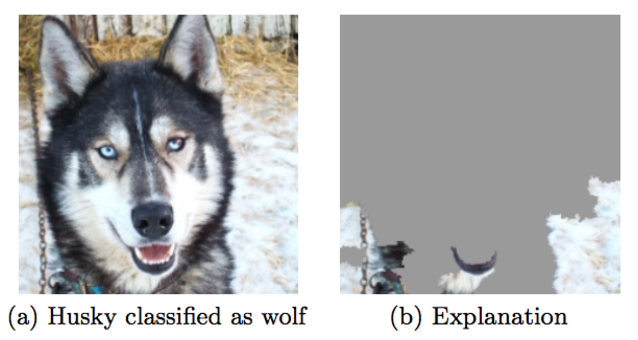
\includegraphics[width=0.6\textwidth]{sketch/husky_explanation}
%
%    \caption[Compact Routing Example]%
%    {Compact Routing\footnote{something} Example}
%  \end{minipage}
%\end{figure}
%

%
% \begin{figure}[!hbt]
%	 		\centering
%			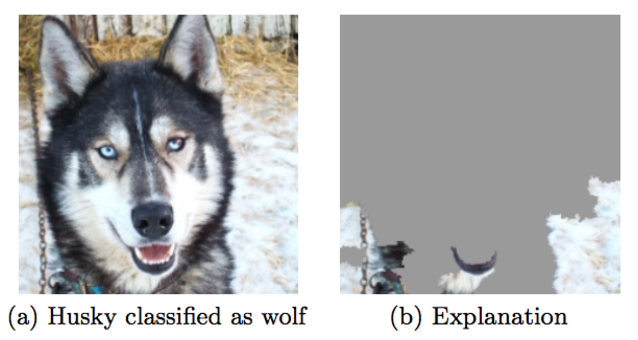
\includegraphics[width=0.6\textwidth]{sketch/husky_explanation}
%			\caption{A classifier classifies ``husky" as ``wolf" because of the snow background.}
%			  \small{ Source : \citep{RibeiroWhyShouldTrust2016} }
%			\label{fig:husky_explanation}
%\end{figure}
%\footnotetext{}


Practically, it is always important to verify whether trained NNs properly utilize data or what information they use to arrive at predictions. From literature, this kind of practical understanding is typically referred to as \textit{explaining} or \textit{interpreting} prediction: NNs are explainable if their predictions can be associated back to what is relevant in the input, in an understandable way. \citet{BachAnalyzingclassifiersFisher2016} demonstrated a case where a NN classifier exploits artifacts in the data to make predictions. In particular, they found that  a classification decision of the NN is primarily based on copyright text in the image. \citet{RibeiroWhyShouldTrust2016} also presented a similar case where a classifier mainly uses background of images to classify between two classes. These discoveries emphasize the importance of having explainable models, not to mention risks associated to human lives from applications powered by them, such as medical diagnosis and autonomous cars.
%
%that nowadays neural networks have been increasingly involved in several aspects of human life, ranging from medical development to self-driving car. 

\subsection{Global and Local Explanation}\label{sec:global_local_explanation}

Formally, there are two aspects of explaining NNs, namely \textit{global} and \textit{local} explanations. Let's consider a NN  classifier categorizing images into $K$ classes.  The global explanation aims to find the most representative image $\patvector{x}^*$ of the class $C_k \in \{C_k\}_{k=1}^K$ in respect to activities of neurons in the network. Activation maximization (AM) \citep{ ErhanUnderstandingRepresentationsLearned2010,SimonyanDeepConvolutionalNetworks2013} is one of the methods in this category. Let's denote $z_{C_k}(\x)$  the score of the class $C_k$ (i.e. pre-softmax activation) of an image $\x$. The objective of AM is to find a synthetic image $\x^*$ such that  

\begin{align*}
\patvector{x}^*  = \patarg{max}{\patvector{x}} z_{C_k}(\x) - \lambda \|\x\|,
\end{align*}
where $\lambda$ is the $L_2$ regularization parameter. \citet{SimonyanDeepConvolutionalNetworks2013} and \citet{NguyenSynthesizingpreferredinputs2016a} demonstrated practical results of AM on state-of-the-art deep neural networks (DNNs).

On the other hand, the local explanation focuses on finding relevant information in $\patvector{x}$ that can explain why the network predicts $\x$ into a certain class $C_k$.  More precisely, this aspect seeks to assign each pixel $x_i \in \patvector{x}$ with a score that quantitatively describes how the pixel influences the decision of the network. The score is formally referred as \textit{relevance score} or \textit{relevance quantity} and denoted with $R_i(\x)$ or $R_i$ if the context is clear. Combining $R_i(\x)$ together will result in what so called, \textit{explanation}, \textit{explanation heatmap}, or \textit{relevance heatmap}.

As illustrated in \addfigure{\ref{fig:comparision_between_global_and_local_analysis}}, the difference between the global and local explanations can be analogously described by formulating questions as follows:
\begin{itemize}
	\item Global explanation : ``How does a typical digit 2 look like?"
    \item Local explanation : ``Which part of the image make it look like a digit 2?" 
\end{itemize}

 \begin{figure}
\centering
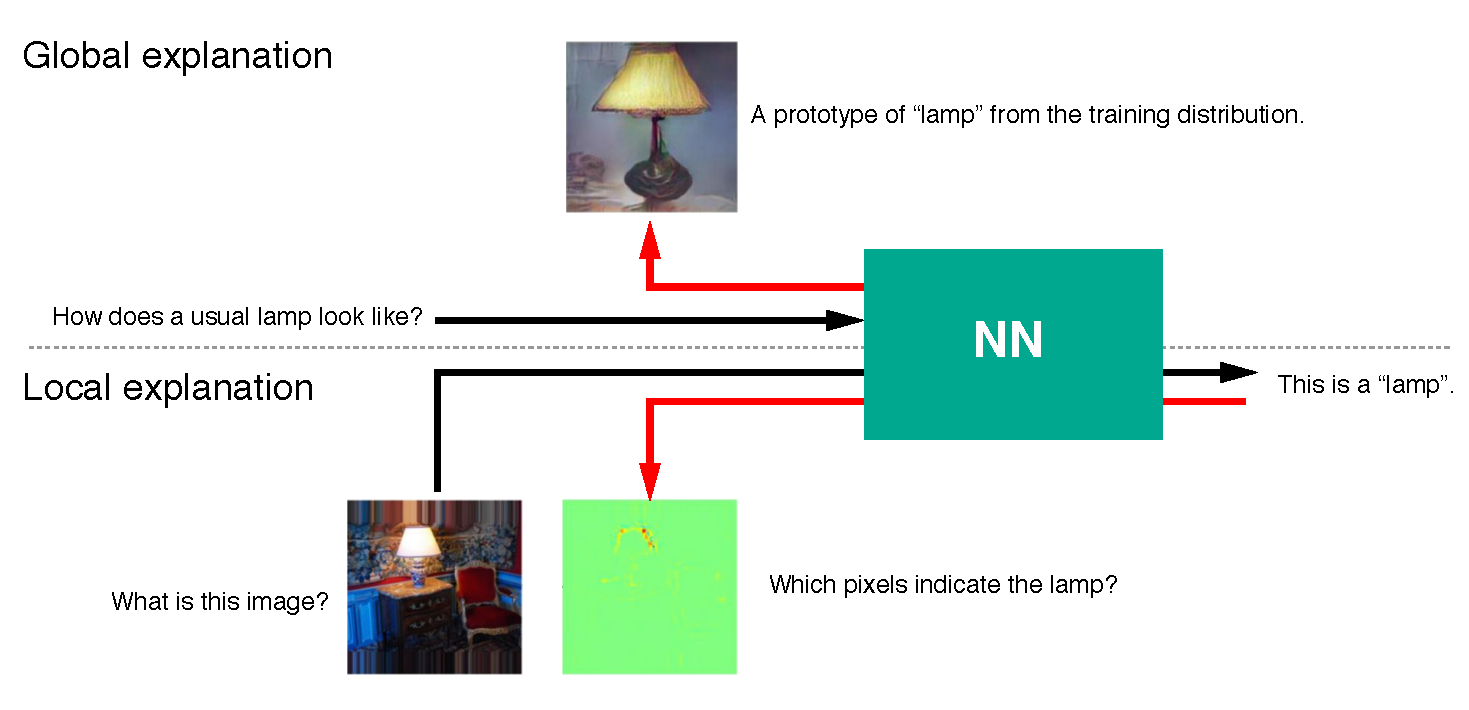
\includegraphics[width=0.8\textwidth]{sketch/global_and_local_method}
\patcaption{Comparison between the global and local explanations.}{Images taken from \citet{MontavonExplainingnonlinearclassification2017}.}
\label{fig:comparision_between_global_and_local_analysis}
\end{figure}

In the following, we are going to discuss several local explanation methods in details and leave content of the global explanation aside due to the scope of the thesis. In particular, we are going to introduce these local explanation methods, namely \textit{sensitivity analysis}, \textit{guided backprop}, \textit{simple Taylor decomposition}, \textit{Layer-wise Relevance Propagation}, and \textit{deep Taylor decomposition}.


%Consider $f(\patvector{x})$ is an output from a neural network classifier that is corresponding to the class prediction, for example the value at the final layer before applying softmax function.
%\begin{definition} Conservation Property
%\begin{align*}
%	\forall \patvector{x} : f(\patvector{x}) = \sum_i R_i
%\end{align*}
%Sum of relevance score of each pixel $x_i$ should equal to the total relevance that the network outputs.
%
%\end{definition}
%\begin{definition} Positivity Property
%\end{definition}
%\begin{definition} Consistency
%\end{definition}

\subsection{Sensitivity Analysis}
\textit{Sensitivity analysis} (SA) is a local explanation technique that derives the relevance score $R_i(\x)$ through the  partial derivative of $\frac{\partial f(\patvector{x})}{ \partial x_i }$.  The method was first proposed by \citet{ZuradaSensitivityAnalysisMinimization1994} in the context of removing redundant input data for a NN. \citet{KhanClassificationdiagnosticprediction2001} applied the technique to investigate a NN trained to classify types of cancer gene expressions. Then, \citet{SimonyanDeepConvolutionalNetworks2013} introduced this technique to a DNN for explaining image classifications. One of the possible formulations is 

\begin{align*}
	R_i(\x) =
	 \bigg( \frac{\partial f(\patvector{x})}{ \partial x_i } \bigg)^2
\end{align*}
	
This formulation is associated to
\begin{align*}
	\sum_i R_i(\x) = \| \nabla f(\patvector{x}) \|^2
\end{align*}

The derivation of $\sum_i R_i(\x)$ above implies that SA seeks to explain $R_i(\x)$ from the aspect of variation magnitudes of $f(\x)$. However, the magnitudes might not reflect the total influence of the input features to the decision.

Practically, this method has a technical advantage because it can be easily implemented in any modern deep learning frameworks, such as TensorFlow \citep{AbadiTensorFlowLargeScaleMachine2016}, via automatic differentiation. Hence, one might consider it as a first tool towards explaining NN decisions.

\subsection{Guided Backpropagation}
\textit{Guided backpropagation} (GB) is an extended version of SA where signals for computing the gradient are propagated throughout the network in a controlled manner. \citet{SpringenbergStrivingSimplicityAll2015a} specifically designed the method for explaining predictions of NNs that rely on ReLU activations.  They first defined an alternative definition  of the ReLU function:
\begin{align*}
	\sigma(h_j) = \underbrace{h_j \mathbbm{1}[ h_j > 0 ]}_{a_j},
\end{align*}
where $\mathbbm{1}[ \cdot ]$  is an indicator function, then they proposed a  propagation rule for the gradient signal passing through a ReLU neuron $j$ as
\begin{align*}
	\frac{\partial_* f(\patvector{x}) }{ \partial h_j } = \mathbbm{1}\bigg[h_j > 0 \bigg] \max \bigg(0, \frac{ \partial_* f(\patvector{x}) }{ \partial a_j } \bigg)
\end{align*}
Applying this rule to the backpropagation yields a signal that is no longer a gradient. However, it can be interpreted as a signal describing positive variations propagated throughout the network. In particular, the rule propagates the incoming signal $\frac{\partial_* f(\x)}{\partial a_j}$, accumulated from successive layers,  to the neuron $j$ only when the signal is positive and the neuron has a positive raw excitation ($h_j > 0$). Similar to SA, we compute the relevance score for each pixel  as 

\begin{align*}
	R_i(\x) = \bigg( \frac{ \partial_* f(\patvector{x}) }{ \partial x_i }  \bigg)^2
\end{align*}

By propagating only positive relevance to only positively activating neurons, \citet{SpringenbergStrivingSimplicityAll2015a} empirically demonstrated that GB produces better explanations than SA in practice. Our results on \addfigure{\ref{fig:lenet_heatmaps}} also confirm this superior.
%
%With this result, one can see that $x_i$ is relevant to the problem if activations $a_j$ that it supplies are active and positively contribute to $f(\patvector{x})$.

\subsection{Layer-wise Relevance Propagation}
The methods introduced so far derive $R_i(\x)$ directly from $f(\patvector{x})$ and do not rely on any knowledge related to the neural network itself, such as network architecture or activation values. Alternatively, \citet{BachPixelWiseExplanationsNonLinear2015} proposed the \textit{layer-wise relevance propagation}(LRP) technique that leverages such information when distributing relevance scores to $x_i$. In particular, LRP propagates relevance scores backward from the last layer to the first layer, similar to the backpropagation algorithm, but just with different quantities.




 \begin{figure}
	\begin{center}
		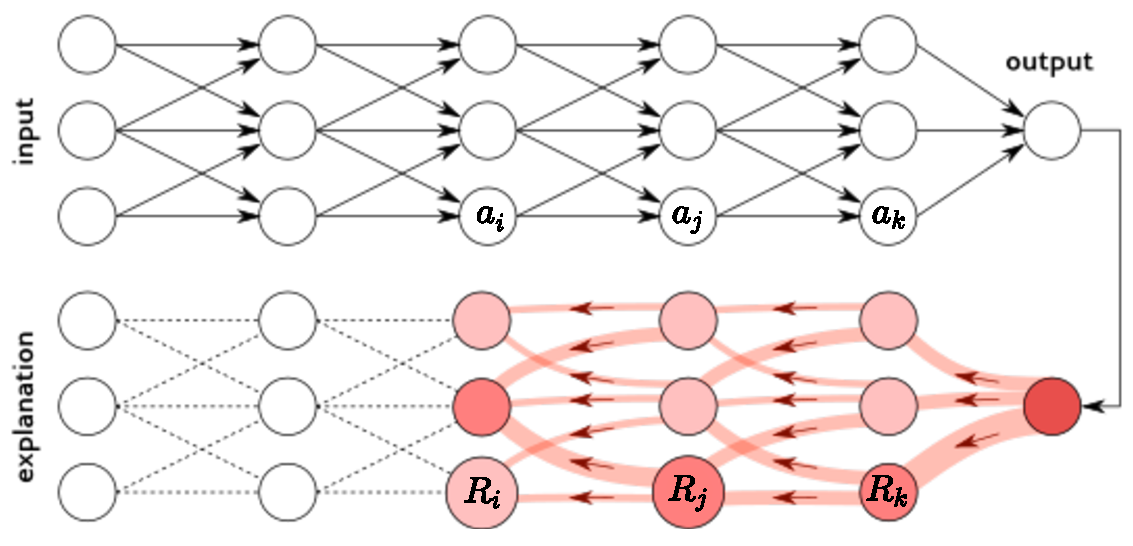
\includegraphics[width=0.5\textwidth]{sketch/lrp_graph}
		\patcaption{An illustration of the relevance propagation in LRP.}{The relevance propagation can be viewed as the backpropagation of relevance quantities. Adapted from \citep{MontavonMethodsinterpretingunderstanding2018}. }
		\label{fig:lrp_graph}
	\end{center}
\end{figure}
%\footnotetext{}}
%}

Let's consider the neural network illustrated in \addfigure{\ref{fig:lrp_graph}}. $R_j$ and $R_k$ are a relevance score of  a neuron $j$ and a neuron $k$ in two successive layers.  LRP has a general relevance propagation rule:

\begin{align} \label{eq:general_lrp_rj}
	R_j = \sum_{k} 	\delta_{j\leftarrow k} R_{k} ,
\end{align}

where $\delta_{j\leftarrow k}$ defines a proportion that  $R_{k}$ contributes to $R_j$. Let's consider further that the activity $a_k$ of the neuron $k$ is computed by 
\begin{align*}
	a_k = \sigma \bigg( \sum_{j} w_{jk} a_j + b_k \bigg),
\end{align*}
where $\sigma$ is an activation function, $w_{jk}$ is the corresponding weight between the two neurons, and $b_k$ is the bias of the neuron $k$. For monotonic increasing $\sigma$, $\delta_{j\leftarrow k}$ can be calculated as follows 
\begin{align} \label{eq:delta_j_k}
	\delta_{j\leftarrow k} = \alpha\frac{a_j w_{jk}^+}{\sum_{j} a_jw_{jk}^+} - \beta\frac{a_j w_{jk}^-}{\sum_{j} a_jw_{jk}^-},
\end{align}
where $w_{jk}^+ = \max(0, w_{jk})$, $w_{jk}^- = \min(0, w_{jk})$, and $\alpha$ and $\beta$ are parameters with $\alpha-\beta = 1$ constraint. Combining (\ref{eq:general_lrp_rj}) and (\ref{eq:delta_j_k}) yields the LRP-$\alpha\beta$ rule:

\begin{align*}
	R_j = \sum_{k} 	\bigg( \alpha\frac{a_j w_{jk}^+}{\sum_{j} a_jw_{jk}^+} - \beta\frac{a_j w_{jk}^-}{\sum_{j} a_jw_{jk}^-} \bigg )  R_{k}
\end{align*}

Algorithm \ref{algo:lrp} summarizes the procedures of the LRP framework, where $(a_j)_j$ is the vector of activations of neurons in a lower-layer $j$ and $(w_{jk})_{jk}$ is the matrix of corresponding weights between neurons in the two layers.

\begin{algorithm}[H]
$f(\patvector{x}), \{ (a_{l_1})_{l_1}, (a_{l_2})_{l_2}, \dots, (a_{l_n})_{l_n}\}$ = \text{forward\_pass}($\patvector{x}, \patvector{\theta}$)\;
$R_k = f(\patvector{x})$\;
 \For{ $\text{layer} \in \text{reverse}(\{l_1, l_2, \dots, l_n\})$}{
$ \text{prev\_layer} \leftarrow \text{layer}  - 1$ \;
	\For{ $j \in $ neurons(prev\_layer), $k \in$ neurons(layer)}{
		$R_j \leftarrow \text{LRP-}\alpha\beta(R_k, (a_j)_j, (w_{jk})_{jk} )$
	}
 }
 \caption{LRP Algorithm}
 \label{algo:lrp}
\end{algorithm}

Alternatively, if we rearrange the rule slightly to 
$$
	R_j = \sum_{k} \bigg( \frac{a_j w_{jk}^+}{\sum_{j} a_jw_{jk}^+} \hat{R}_{k} + \frac{a_j w_{jk}^-}{\sum_{j} a_jw_{jk}^-} \check{R}_{k} \bigg),
$$ 
where $\hat{R}_{k}  = \alpha R_{k}$ and  $\check{R}_{k} = -\beta R_{k} $. We can then intuitively interpret this propagation as 

\begin{quote}
``Relevance $\hat{R}_k$'' should be redistributed to the lower-layer neurons $(a_j)_j$ in proportion to their excitatory effect on $a_k$. ``Counter-relevance'' $\check{R}_k $ should be redistributed to the lower-layer neurons $(a_j)_j$ in proportion to their inhibitory effect on $a_j$
	- Section 5.1 \citep{MontavonMethodsinterpretingunderstanding2018}
\end{quote} 

Moreover, LRP  has a \textit{conservation property} in which the total relevance quantity is conserved during propagating $f(\patvector{x})$ to $R_i(\x)$. This property is similar to a principle applied in \citep{PoulinVisualExplanationEvidence2006,LandeckerInterpretingindividualclassifications2013} where they developed explanation techniques for other types of ML models. Formally, the conservation property is 
\begin{align*}
	\sum_{i} R_i =  \cdots =	\sum_{j} R_j = \sum_{k} R_k = \cdots = f(\patvector{x})
\end{align*}

Nonetheless, choosing values of $\alpha$ and $\beta$ is still a question for LRP.  In particular, \citet{MontavonExplainingnonlinearclassification2017} and \citet{BinderLayerWiseRelevancePropagation2016} demonstrated that the influence of the values to the quality of explanations  depends on the architecture of the network being explained. For example, \cite{MontavonMethodsinterpretingunderstanding2018} observed that LRP-${\alpha_1\beta_0}$ works well for deep architectures, such as GoogleNet \citep{SzegedyGoingdeeperconvolutions2015}, while LRP-${\alpha_2\beta_1}$ is better for shallower architectures, such as BVLC CaffeNet \citep{JiaCaffeConvolutionalArchitecture2014}.

\subsection{Simple Taylor Decomposition}
As the name suggested,  the method decomposes $f(\patvector{x})$ using the Taylor expansion around a root point $\tilde{\patvector{x}}$. \citet{BazenTaylorDecompositionUnified2013} introduced  the technique to explain marginal effects in econometric models. \citet{BachPixelWiseExplanationsNonLinear2015} applied the technique to a pixel-wise decomposition method for explaining non-linear classification predictions. The relevance scores $(R_i(\x))_i$ are interpreted as the first order terms of the Taylor series. Formally, the decomposition is 


\begin{align} \label{eq:simple_taylor_expansion}
	f(\patvector{x}) 	&= f(\tilde{\patvector{x}}) + \sum_{i} \underbrace{\frac{\partial f }{ \partial x_i } \Bigg|_{\tilde{\patvector{x}}}  ( x_i - \tilde{x}_i ) }_{R_i} + \zeta, 
\end{align}
where $\zeta$ are the second and higher order terms of the Taylor series. The root point $\tilde{\patvector{x}}$ can be found via the optimization below 
\begin{align*}
\tilde{\patvector{x}} = \underset{\patvector{\xi} \in \mathcal{X} }{\text{argmin}}  \| \patvector{\xi} - \patvector{x} \|^2 \hspace{1cm}  \text{s.t.}\  f(\patvector{\xi}) = 0,
\end{align*}
where $\mathcal{X}$ represents the distribution of possible input. This optimization is time-consuming  and the root point $\tilde{\patvector{x}}$ might potentially diverge from the input sample $\patvector{x}$ leading to  non-informative scores $(R_i)_i$. However, $\tilde{\patvector{x}}$ can be computed analytically for NNs using piece-wise linear activations (e.g. ReLU). With the assumptions of 1) $\sigma(tx) = t\sigma(x) ,\forall t \ge 0$ and 2) no use of bias, \citet{MontavonMethodsinterpretingunderstanding2018} particularly argued that  the root point $\tilde{\patvector{x}}$ can be found approximately in the same flat region as $\patvector{x}$, $\tilde{\patvector{x}} = \underset{\epsilon \rightarrow 0 }{\lim} \epsilon \x$, yielding

\begin{align*}
	\frac{\partial f(\patvector{x})}{\partial x_i}\bigg|_{\tilde{\patvector{x}}} = \frac{\partial f(\patvector{x})}{\partial x_i}\bigg|_{\patvector{x}} 
\end{align*}

%demonstrate that  neural networks whose activations $\sigma(x)$ are piecewise linear functions  with , for example a deep Rectified Linear Unit (ReLU) network without biases, 
%
As a result, (\ref{eq:simple_taylor_expansion}) can be simplified to
\begin{align}
	f(\patvector{x}) &= \sum_{i} \frac{\partial f(\patvector{x})}{\partial x_i}\bigg|_{\patvector{x}}  x_i \nonumber \\
	R_i &= \frac{\partial f(\patvector{x})}{\partial x_i}\bigg|_{\patvector{x}}  x_i \label{eq:simple_r_i}
\end{align}

This derivation shows a relationship between SA and simple Taylor decomposition. Specifically, $R_i$ will have a high value if $x_i$ highly activates and its variation positively affects $f(\x)$ and vice versa.


\subsection{Deep Taylor Decomposition}


Deep Taylor decomposition (DTD) is another local explanation technique that relies on the Taylor expansion. Unlike simple Taylor decomposition, DTD instead decomposes the relevance score $R_k$ into the relevance scores $(R_{j \leftarrow k})_j$ of neurons in the lower-layer $j$ using the Taylor expansion around a root point $(\tilde{a}_j)_j$. \cite{MontavonExplainingnonlinearclassification2017} proposed the method to explain decisions of NNs with piece-wise linear activations (i.e., ReLU). Similar to the LRP method, DTD successively propagates relevance scores  $(R_k)_k$ to $(R_j)_j$ in the previous layer. The process is repeated until arriving at the relevance scores of the input layer $(R_i(\x))_i$.

 Let's denote $(a_j)_j$ the vector of neuron activations in the layer $j$. $R_k$ is formally decomposed as follows


% In fact, it can be shown that LRP's propagation rule is equivalent to one of DT's rules.


 \begin{align} \label{eq:tl_rj}
 R_k = R_k \bigg|_{ (\tilde{a}_j)_j } + \sum_{ j } 	\frac{\partial  R_k }{ \partial a_j } \bigg|_{ (\tilde{a}_j)_j } ( a_j - \tilde{a}_j ) + \zeta_k,
 \end{align}
 where $\zeta_k$ are the second and higher order terms of the Taylor series.

Let's assume further that the second and higher terms $\zeta_k = 0 $ and there exists a root point $(\tilde{a}_j)_j$ that $R_k = 0$. Then, (\ref{eq:tl_rj}) can be reduced to
\begin{align*}
 R_k = \sum_{ j } \underbrace{	\frac{\partial  R_k }{ \partial a_j } \bigg|_{ (\tilde{a}_j)_j }  ( a_j - \tilde{a}_j ) }_{ R_{j \leftarrow k } }
\end{align*}

Hence, the relevance score $R_j$ of a neuron $j$ is 
$$ R_j = \sum_{k} R_{j\leftarrow k}$$

Given the result, one can show that DTD also has the  \textit{conservation property}:
\begin{align} 
	R_j &= \sum_{k} R_{j\leftarrow k} \nonumber \\
\sum_{j}	R_j &= \sum_{j} \sum_{k} R_{j\leftarrow k} \nonumber\\
%\sum_{j}	R_j &= \sum_{k} \sum_{j} R_{j\leftarrow k} \nonumber \\
\sum_{j}	R_j &= \sum_{k}  R_{k} \nonumber \\
\sum_i 	R_{i} = 	\dots = \sum_j R_{j} &= \sum_k R_{k} = \dots =  f(\patvector{x}) \nonumber
\end{align}

%Demonstrated by \cite{MontavonExplainingnonlinearclassification2017}, Equation \ref{eq:rj_equal_rk} holds for all $j, k$ and all subsequent layers. Hence, this results in  conservation property which guarantee that no relevance loss during the propagations.
%\begin{align}
%\sum_i 	R_{i} = 	\dots = \sum_j R_{j} = \sum_k R_{k} = \dots =  f(\patvector{x})
%\end{align}
 
 
%\begin{figure}[h]
%\centering
%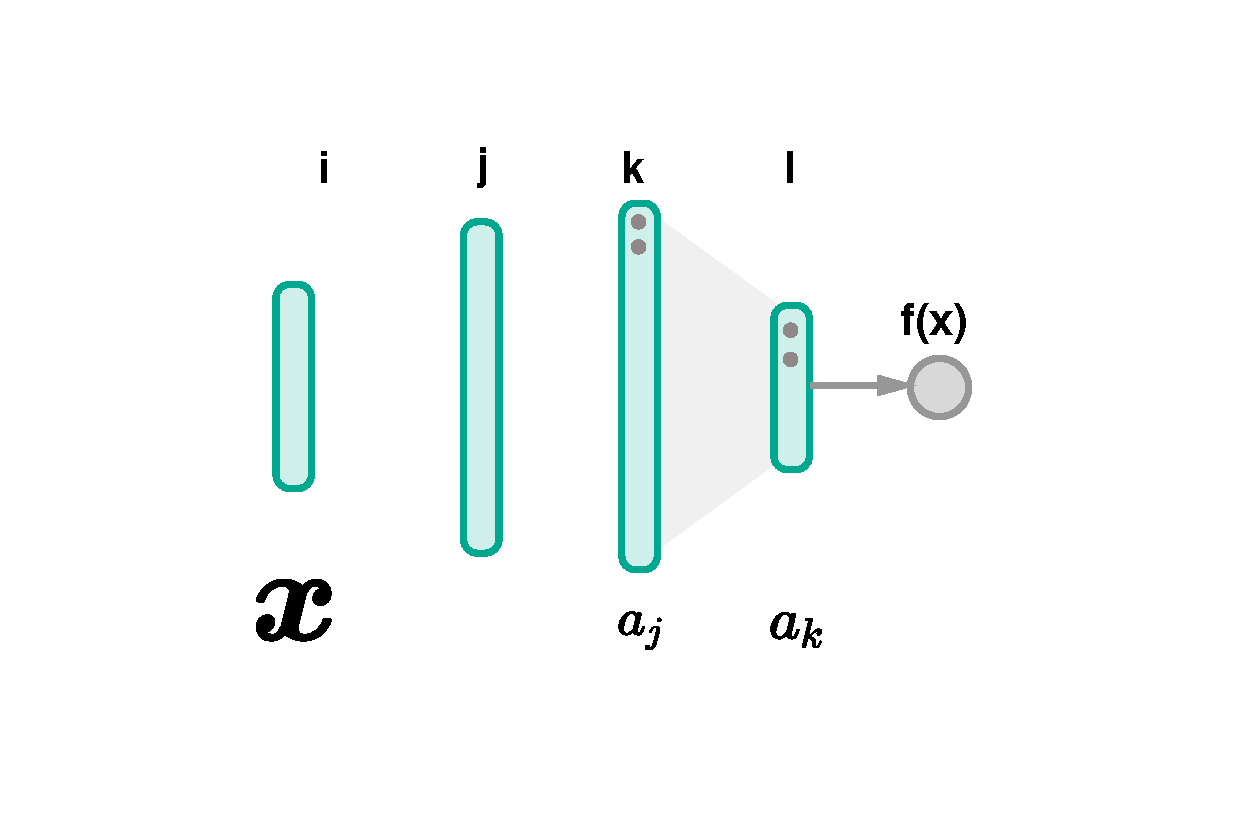
\includegraphics[width=0.8\textwidth]{sketch/deep_tayloy_decomposition_toy}
%\caption{A Simple network}
%\label{fig:deep_tayloy_decomposition_toy}
%\end{figure}

\subsubsection{Finding the root point} 
Let's consider a NN whose $R_k$ is computed via the ReLU function:
% is based on activations of $a_j$ in the previous layer and  :
\begin{align}\label{eq:r_k_deep_taylor}
R_k = \text{max}\ \bigg(0, \sum_{j} a_j w_{jk}  + b_k \bigg),
\end{align}
where $b_k$ is kept to be strictly non-positive (i.e. $b_k < 0$). Using the ReLU function results in $\xi_k=0$.

To find a root point $(\tilde{a}_j)_j$, one can see that  there are  two cases to be considered, namely when $R_k = 0$ and $R_k > 0$. Trivially, $(a_j)_j$ is already the root point when $R_k=0$. For the latter, the root point can be found by performing  line search in  a direction $(v_j)_j$ with magnitude $t$:
\begin{align}\label{eq:root_aj_aj}
\tilde{a}_j = a_j - t v_j,
\end{align}
More precisely, the root point is at the intersection point between (\ref{eq:r_k_deep_taylor}) and (\ref{eq:root_aj_aj}) where $R_k=0$. Hence,
\begin{align*}
  0 &= 	\sum_{j} (a_j - t v_j) w_{jk}  + b_k\\
%  0 &= \sum_{j} a_j w_{jk} - t v_j w_{jk}  + b_k\\
%  t \sum_{j} v_j w_{jk} &= R_k \\
  t &= \frac{R_k}{\sum_{j} v_j w_{jk}}
\end{align*}

Therefore, $R_j$ can be then calculated by
\begin{align*}
R_j &= \sum_k	\frac{\partial  R_k }{ \partial a_j } \bigg|_{ (\tilde{a}_j)_j }  ( a_j - \tilde{a}_j ) \\
&=	\sum_k w_{jk} tv_j \\
&=	\sum_k \frac{ v_j w_{jk}   }{\sum_{j} v_j w_{jk}}  R_k
\end{align*}

%\begin{figure}[!hbt]
%\centering
%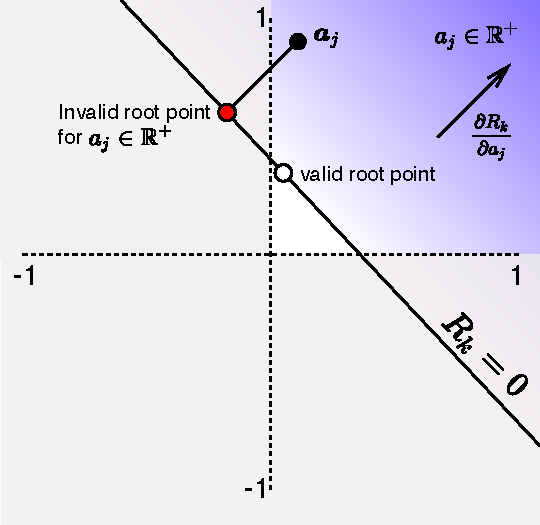
\includegraphics[width=0.4\textwidth]{sketch/invalid_root_point_example}
%\caption{Function's view of $R_k$  and root point candidates}
%\label{fig:root_point_illus}
%\end{figure}



The last step is to find $(v_j)_j$ such that $(\tilde{a}_j)_j$ is the closest point to the line $R_k=0$ with the constraint that $\tilde{a}_j$ needs to be in the same domain as $a_j$. For example, if $a_j \in \mathbb{R}^+$, then $\tilde{a}_j$ must be also in $\mathbb{R}^+$. \addfigure{\ref{fig:dtd_rule_cases}} illustrates the intuition.  Therefore, $(v_j)_j$ needs to be separately derived for each domain of $a_j$. In particular, there are two possible domains to be considered, namely 
%\begin{enumerate}
%\item $a_j \in \setreal$  \\
%	For this domain, the search direction is just the direction of derivative $\frac{\partial R_k}{ \partial a_j }$. Hence, 
%\begin{align*}
%	R_j &=	\sum_k \frac{ w_{jk}^2  }{\sum_{j} w_{jk}^2}  R_k
%\end{align*}
%\item $a_j \in \setreal^+$ :
%\item $a_j \in [l_j , h_j]$ where $l_j \le 0 < h_j $ :
%\end{enumerate}
%
% of $\patvector{a}_j$.

\begin{figure}
\centering

\subfloat[$a_j \in \setreal^+$\label{fig:dtd_zplus}]{%
       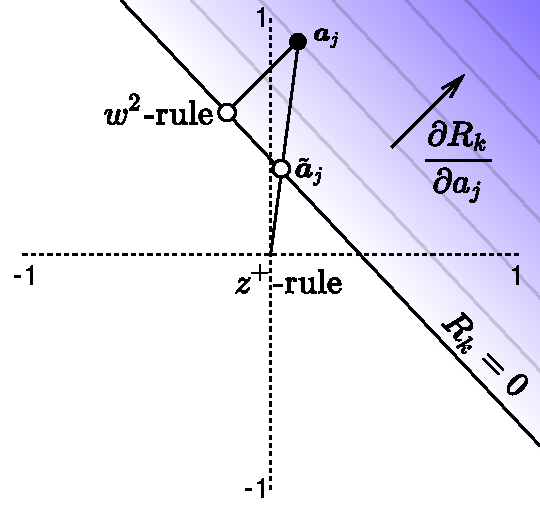
\includegraphics[width=0.4\textwidth]{sketch/zplus_rule_case_1}
}
     \hfill
\subfloat[ {$a_j \in [l_j , h_j ] $ } where $l_j \le 0 < h_j $   \label{fig:dtd_zbeta}]{%
       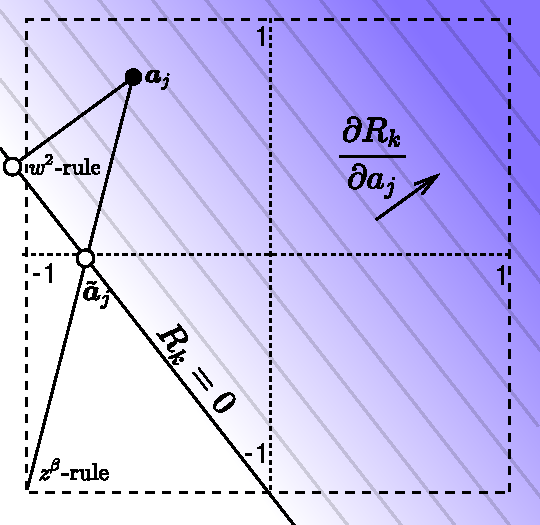
\includegraphics[width=0.4\textwidth]{sketch/zbeta_rule_case_1}
}

\patcaption{Two functional  views of $R_k$ for different domains of $a_j$.}{The DTD root points are the red circles, while the nearest roots in the unconstrained space are the white ones. Blue indicates a high function value, while white indicates a low value. The grey area indicates a invalid region. Adapted from \citep{MontavonExplainingnonlinearclassification2017}. }
\label{fig:dtd_rule_cases}
\end{figure}


%\subsubsection{Case $a_j \in \mathbb{R}$ : $w^2$-rule}
%
%Trivially, the search direction $v_j$ is just the direction of derivative $\frac{\partial R_k}{ \partial a_j }$. This yields the $w^2$-rule:
%
%\begin{align*}
%	R_j &=	\sum_k \frac{ w_{jk}^2  }{\sum_{j} w_{jk}^2}  R_k
%\end{align*}

\subsubsection{Case $a_j \in \mathbb{R}^+$ : $z^+$-rule}

The ReLU activation results $a_j$ in this domain. According to \addfigure{\ref{fig:dtd_zplus}}, the DTD root point of this domain can be found on the line segment  $( (a_j \mathbbm{1}[ w_{jk}  < 0 ])_j, (a_j)_j )$. Hence, the search direction is 
\begin{align*}
	v_j &= a_j - a_j \mathbbm{1}[ w_{jk}  < 0 ] \\
	&= a_j \mathbbm{1}[ w_{jk}  \ge 0 ]
\end{align*}
This yields $z^+$-rule:
\begin{align*}
		R_j &=	\sum_k \frac{ w_{jk} a_j \mathbbm{1}[w_{jk}  \ge 0 ]  }{\sum_{j} w_{jk} a_j \mathbbm{1}[ w_{jk}  \ge 0 ]}  R_k\\
		&=	\sum_k  \frac{ a_j  w_{jk}^+   }{\sum_{j}  a_j w_{jk}^+  }R_k,
\end{align*}
where $w_{jk}^+= \max(0, w_{jk})$. Interestingly, this propagation rule is equivalent to LRP-$\alpha_1\beta_0$. 


\subsubsection{Case $a_j \in [l_j , h_j]$ where $l_j \le 0 < h_j $ : $z^\mathcal{B}$-rule}

This propagation rule is for layers that their incoming activations are bounded, for example the first layer of NNs that receives pixel intensities as input. As shown in \addfigure{\ref{fig:dtd_zbeta}}, the root point is on the line segment $( (l_j \mathbbm{1}[ w_{jk}  > 0 ]  + h_j \mathbbm{1}[ w_{jk}  < 0 ])_j  , (a_j)_j ) $. Hence,  the search direction is 
\begin{align*}
	v_j &= a_j - \tilde{a}_j \\
	&=a_j  - l_j \mathbbm{1}[ w_{jk}  > 0 ]  - h_j \mathbbm{1}[ w_{jk}  < 0 ]
\end{align*}
This search direction results in  $z^\mathcal{B}$-rule:
\begin{align*}
		R_j &=	\sum_k \frac{ w_{jk}  (a_j  - l_j \mathbbm{1}[ w_{jk}  > 0 ]  - h_j \mathbbm{1}[ w_{jk}  < 0 ]) }{\sum_{j} w_{jk}  (a_j  - l_j \mathbbm{1}[ w_{jk}  > 0 ] - h_j \mathbbm{1}[ w_{jk}  < 0 ]) }  R_k\\
		&=	\sum_k  \frac{ a_j  w_{jk} - l_j w_{jk}^+ - h_j w_{jk}^-  }{\sum_{j}   a_j  w_{jk} - l_j w_{jk}^+ - h_j w_{jk}^- }  R_k,
\end{align*}
where $w_{jk}^- = \min(0, w_{jk})$.

Applying these propagation rules accordingly with LRP Algorithm \ref{algo:lrp} yields deep Taylor decomposition of  $f(\x)$. These are brief derivations of the DTD propagation rules. More theoretical details can be found in the original paper \citep{MontavonExplainingnonlinearclassification2017}.



%\renewcommand{\arraystretch}{1}
%\begin{table}[h]
%\centering
%\begin{tabular}{|l|l|}
%\hline
%\multicolumn{1}{|c|}{Rule and input domain} & \multicolumn{1}{c|}{Formula} \\ \hline
%$w^2$-rule : Real values,  $a_j \in \mathbb{R}$ & \parbox{1cm}{
%	\begin{align*}
%		R_j =	\sum_k \frac{ w_{jk}^2  }{\sum_{j} w_{jk}^2}  R_k  	
%    \end{align*}}
% \\ \hline
%% &                                \\ \hline
%$z^+$-rule : ReLU activations, $a_j \in \mathbb{R}^+$    & \parbox{1cm}{\begin{align*}
%R_j = \sum_k  \frac{ a_j  w_{jk}^+   }{\sum_{j}  a_j w_{jk}^+  }  R_k	
%\end{align*}} \\ \hline
%$z^\beta$-rule : Pixel Intensities, $ a_j \in [l_j , h_j]$ where $l_j \le 0 < h_j $  & \parbox{1cm}{\begin{align*}
%R_j = \sum_k  \frac{ a_j  w_{jk} - l_j w_{jk}^- - h_j w_{jk}^+  }{\sum_{j}   a_j  w_{jk} - l_j w_{jk}^- - h_j w_{jk}^+ }  R_k	
%\end{align*}}
%               \\ \hline
%\end{tabular}
%\caption{Relevance propagation rules of deep Taylor decomposition. }
%\label{tab:lrp_deep_taylor_rules}
%\end{table}
%\renewcommand{\arraystretch}{1}


\begin{figure}[!htb]
\centering
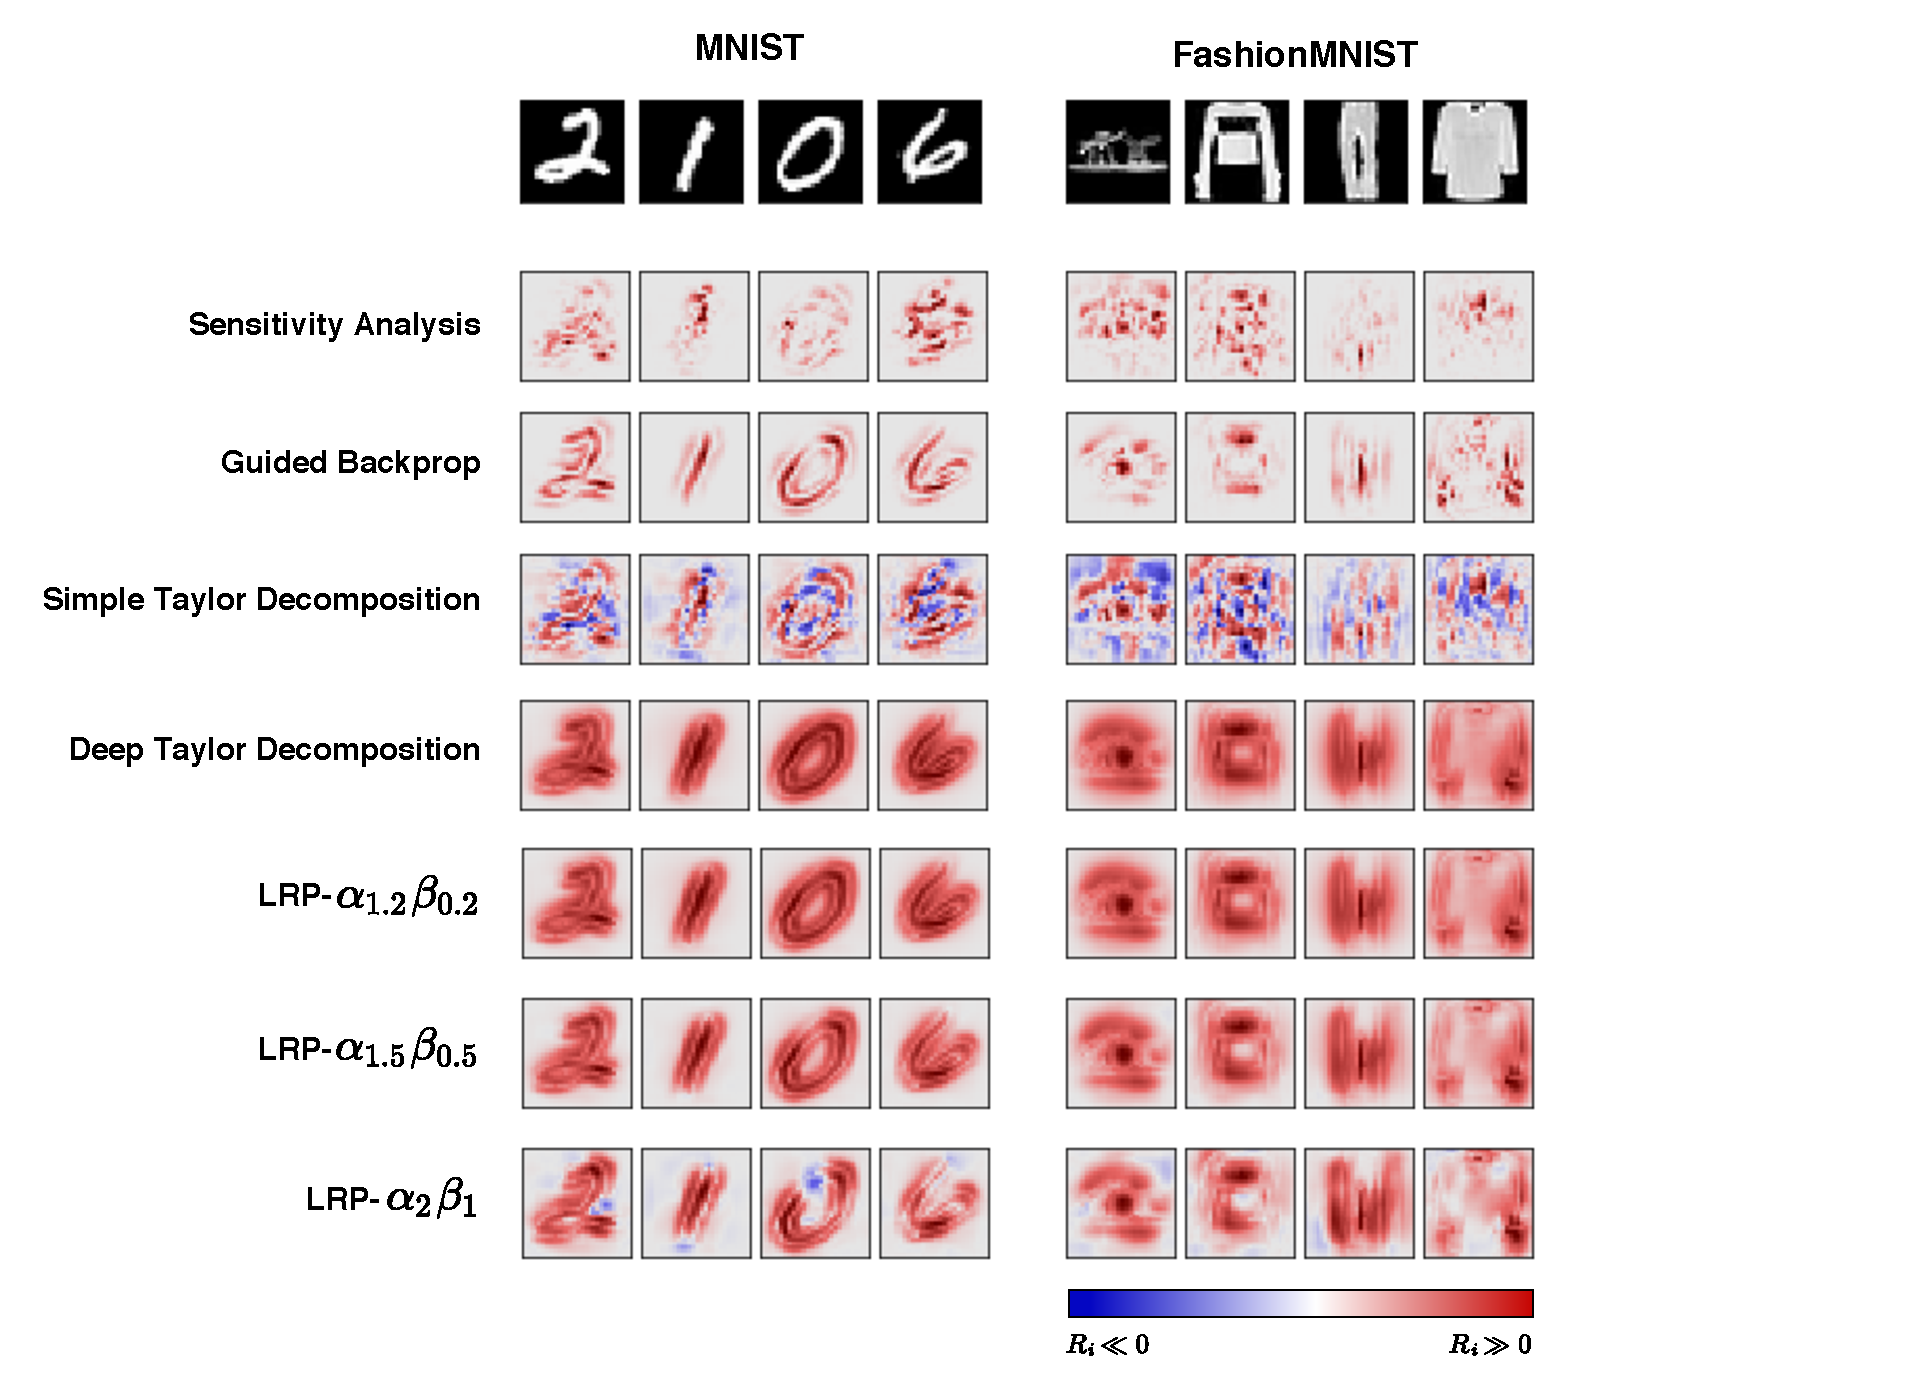
\includegraphics[width=\textwidth]{sketch/lenet_heatmaps}
\patcaption{Relevance heatmaps produced by different explanation methods explaining classification decisions of LeNet-5 on MNIST and FashionMNIST datasets.}{\heatmapscaleexplain }
\label{fig:lenet_heatmaps}
\end{figure}

In this section, we have described the intuition and the details of several local explanation methods. \addfigure{\ref{fig:lenet_heatmaps}} shows  examples of relevance heatmaps from those methods in explaining classification decisions of the LeNet-5 \citep{LeCunGradientBasedLearningApplied2001} architecture. We train the networks with 100 epochs, batch size 50, and dropout probability 0.2. The trained models achieve accuracy at 99.21\% for MNIST and 87.90\% for FashionMNIST. 

From \addfigure{\ref{fig:lenet_heatmaps}}, we can also see general characteristics of explanation heatmap from each method. In particular, one can observe that simple Taylor decomposition provides the most noisy and less informative explanations, while the ones from sensitivity analysis (SA)  look less noisy and contain some structures of the input. Guided backprop (GB), deep Taylor decomposition (DTD), and layer-wise relevance propagation (LRP) produce smoother and more informative explanations. It is worth noting that DTD and LRP methods produce similar relevance heatmaps when $\beta$ is small. Given this result, we are going to consider SA, GB, DTD, and $\lrpp$ in the following experiments.